\section{Kinematic Equations of Motion}
The kinematic equations of motion and the dynamic equations of motion are the two types of equations of motion in attitude dynamics. Kinematics is the study of motion in general, regardless of the forces that derive it. The kinematic equations of motion are a set of first-order differential equations that describe how the attitude parameters change with time. The dynamic equations of motion will be developed, which express the time dependence of $\boldsymbol{\omega}$.

\subsection{Time Derivative of Quaternions}
Let $q(t)$ be a unit quaternion function of time, and $\boldsymbol{\omega}(t)$ the angular velocity determined by $q(t)$. The derivative of $q(t)$ is
\begin{equation}\label{eqn:6.1}
    \dot{\mathbf{q}}=\frac{1}{2}q\boldsymbol{\omega}
\end{equation}
At $t+\Delta t$, the rotation is described by $q(t+\Delta t)$. This is after some extra rotation during $\Delta t$ achieved on the frame that has already experienced a rotation described by $q(t)$. This extra rotation is about the instantaneous axis $\widehat{\boldsymbol{\omega}}=\frac{\boldsymbol{\omega}}{\|\boldsymbol{\omega}\|}$ over the angle $\Delta \theta=\|\boldsymbol{\omega}\| \Delta t$. With the aid off equation \ref{eqn:sin_cos}, it can be expressed as
\begin{equation}
  \Delta \mathbf{q}=\cos \frac{\theta}{2}+\widehat{\boldsymbol{\omega}} \sin \frac{\theta}{2}  
\end{equation}
\begin{equation}
\Delta \mathbf{q}=\cos \frac{\|\boldsymbol{\omega}\| \Delta t}{2}+\frac{\boldsymbol{\omega}}{\|\boldsymbol{\omega}\|} \sin \frac{\|\boldsymbol{\omega}\| \Delta t}{2}    
\end{equation}
Inferring,
\begin{equation}
\begin{aligned}
\mathbf{q}(t+\Delta t)&=\Delta \mathbf{q} \mathbf{q}(t) \\
\mathbf{q}(t+\Delta t)-q(t)&=\left(\cos \frac{\|\boldsymbol{\omega}\| \Delta t}{2}+\frac{\boldsymbol{\omega}}{\|\boldsymbol{\omega}\|} \sin \frac{\|\boldsymbol{\omega}\| \Delta t}{2}\right) \mathbf{q}-\mathbf{q} \\
&=\left(-2 \sin ^{2} \frac{\|\boldsymbol{\omega}\| \Delta t}{4}+\frac{\boldsymbol{\omega}}{\|\boldsymbol{\omega}\|} \sin \frac{\|\boldsymbol{\omega}\| \Delta t}{2}\right) \mathbf{q}
\end{aligned}    
\end{equation}
Divide by $\Delta t$
\begin{equation}
    \frac{\mathbf{q}(t+\Delta t)-\mathbf{q}(t)}{\Delta t}=\frac{\left(-2 \sin ^{2} \frac{\|\boldsymbol{\omega}\| \Delta t}{4}+\frac{\boldsymbol{\omega}}{\|\boldsymbol{\omega}\|} \sin \frac{\|\boldsymbol{\omega}\| \Delta t}{2}\right) \mathbf{q}}{\Delta t}
\end{equation}
\begin{equation}
    \dot{\mathbf{q}}=\lim _{\Delta t \rightarrow 0} \frac{q(t+\Delta t)-\mathbf{q}(t)}{\Delta t}=\lim _{\Delta t \rightarrow 0} \frac{1}{\Delta t}\left(-2 \sin ^{2} \frac{\|\omega\| \Delta t}{4}+\frac{\omega}{\|\omega\|} \sin \frac{\|\omega\| \Delta t}{2}\right) \mathbf{q}
\end{equation}
\begin{equation}
    =\frac{\omega}{\|\boldsymbol{\omega}\| \Delta t \rightarrow 0} \lim _{\Delta t} \frac{1}{\Delta t}\left(\sin \frac{\|\omega\| \Delta t}{2}\right) q=\frac{\boldsymbol{\omega}}{\|\boldsymbol{\omega}\|}\left(\frac{\|\omega\| \Delta t}{2}\right) \mathbf{q}
\end{equation}
\[\boxed{
\dot{\mathbf{q}}=\frac{1}{2} \boldsymbol{\omega} \mathbf{q}
}\]
Which matches equation \ref{eqn:6.1}.
Proposing $\boldsymbol{\omega}$ as a pure quaternion $\boldsymbol{\omega}=\left[\begin{array}{llll}0 & \omega_{1} & \omega_{2} & \omega_{3}\end{array}\right]^{T} \in \mathbb{H}$ and from quaternion multiplication discussed earlier
\begin{equation}
    \dot{\mathbf{q}}=\frac{1}{2}\left[\begin{array}{c}
-\omega_{1} q_{1}-\omega_{2} q_{2}-\omega_{3} q_{3} \\
\omega_{1} q_{0}+\omega_{2} q_{3}-\omega_{3} q_{2} \\
\omega_{2} q_{0}+\omega_{3} q_{1}-\omega_{1} q_{3} \\
\omega_{3} q_{0}+\omega_{1} q_{2}-\omega_{2} q_{1}
\end{array}\right]
\end{equation}

\subsection{The Omega operator}
Let the omega operator $\boldsymbol{\Omega}(\boldsymbol{\omega})$ be
\begin{equation}
    \boldsymbol{\Omega}(\boldsymbol{\omega})=\left[\begin{array}{cc}
    0 & -\boldsymbol{\omega}^{T} \\
    \boldsymbol{\omega} & \lfloor\boldsymbol{\omega}\rfloor_{\times}
    \end{array}\right]  
\end{equation}
Where the expression $\lfloor\boldsymbol{\omega}\rfloor_{\times}$expands a vector $\boldsymbol{\omega} \in \mathbb{R}^{3} \subset \mathbb{H}$ into a skew-symmetric matrix as
\begin{equation}
    \lfloor\boldsymbol{\omega}\rfloor_{\times} \triangleq\left[\begin{array}{ccc}
    0 & -\omega_{2} & \omega_{1} \\
    \omega_{2} & 0 & -\omega_{0} \\
    -\omega_{1} & \omega_{0} & 0
    \end{array}\right]
\end{equation}
So, the $\boldsymbol{\Omega}(\boldsymbol{\omega})$ will be
\begin{equation}
    \boldsymbol{\Omega}(\boldsymbol{\omega})=\left[\begin{array}{cccc}
    0 & -\omega_{1} & -\omega_{2} & -\omega_{3} \\
    \omega_{1} & 0 & \omega_{2} & -\omega_{1} \\
    \omega_{2} & -\omega_{2} & 0 & \omega_{0} \\
    \omega_{3} & \omega_{1} & -\omega_{0} & 0
    \end{array}\right]
\end{equation}
An equivalent matrix expression for the derivative of the quaternion is
\begin{equation}
    \dot{\mathbf{q}}=\frac{1}{2} \boldsymbol{\Omega}(\boldsymbol{\omega}) \mathbf{q}=\frac{1}{2}\left[\begin{array}{cccc}
    0 & -\omega_{1} & -\omega_{2} & -\omega_{3} \\
    \omega_{1} & 0 & -\omega_{3} & \omega_{2} \\
    \omega_{2} & \omega_{3} & 0 & -\omega_{1} \\
    \omega_{3} & -\omega_{2} & \omega_{1} & 0
    \end{array}\right]\left[\begin{array}{l}
    q_{0} \\
    q_{1} \\
    q_{2} \\
    q_{3}
    \end{array}\right]=\left[\begin{array}{c}
    -\omega_{1} q_{1}-\omega_{2} q_{2}-\omega_{3} q_{3} \\
    \omega_{1} q_{0}-\omega_{3} q_{2}+\omega_{2} q_{3} \\
    \omega_{2} q_{0}+\omega_{3} q_{1}-\omega_{1} q_{3} \\
    \omega_{3} q_{0}-\omega_{2} q_{1}+\omega_{1} q_{2}
    \end{array}\right]
\end{equation}
This definition simplifies the quaternion multiplication as it only involves simple matrix algebra. 
\section{Angular Momentum and Moment of Inertia Tensor}
Consider the case of a rigid body traveling in an inertial frame. The transnational motion of the body's center of mass combined with a rotational motion of the body along some axis via its center of mass can be used to characterize this motion.

The angular momentum $\boldsymbol{h}$ about the center of mass of a rigid body consists of $m_{n}$ objects is
\begin{equation}
\boldsymbol{h}=\sum_{m_{n}} \boldsymbol{r}_{\boldsymbol{n}} \times\left(\boldsymbol{\omega} \times \boldsymbol{r}_{\boldsymbol{n}}\right) m_{n}    
\end{equation}

If the vector part of $\boldsymbol{\omega}=\left[\begin{array}{lll}\omega_{x} & \omega_{y} & \omega_{z}\end{array}\right]^{T}$ is the angular velocity vector describing the motion of the rigid body, the angular momentum vector is defined as, see \cite{sidi1997spacecraft}.
\begin{equation}
\boldsymbol{h}=\left[\begin{array}{ccc}
I_{x x} & -I_{x y} & -I_{x z} \\
-I_{y x} & I_{y y} & -I_{y z} \\
-I_{z x} & -I_{z y} & I_{z z}
\end{array}\right]\left[\begin{array}{l}
\omega_{x} \\
\omega_{y} \\
\omega_{z}
\end{array}\right]=[\mathbf{I}] \boldsymbol{\omega}    
\end{equation}
$[\mathbf{I}]$ is the inertia tensor.

\section{Dynamics Equation of Motion}
\subsection{Euler’s Moment Equation}
The angular momentum equation of a rigid body about its center of mass is simply given as
\begin{equation}
\boldsymbol{M}=\dot{\boldsymbol{h}}    
\end{equation}
Where $\boldsymbol{h}$ is the angular momentum vector of a rigid body about its mass center, $\boldsymbol{M}$ is the external moment acting on the body about its mass center.

We will utilize the well-known operator equation operating on a given vector A in the following analysis.
\begin{equation}
\frac{d}{d t} \boldsymbol{A}_{I}=\frac{d}{d t} \boldsymbol{A}_{B}+\boldsymbol{\omega} \times \boldsymbol{A}
\end{equation}
This simply says that the rate of change of the vector $\boldsymbol{A}$ in the stationary coordinate system \textit{$I$ "inertial" in our instance} equals the rate of change of the vector $\boldsymbol{A}$ in the rotating coordinate system \textit{B-"body"} plus the vector product $\boldsymbol{\omega} \times \boldsymbol{A}$. This relation will be used along the discussion

The rotational equation of motion of a rigid body about its center of mass is then written as
\begin{equation}
\boldsymbol{M}=\boldsymbol{h}_{n}=\left\{\frac{d \boldsymbol{h}}{d t}\right\}_{B}+\boldsymbol{\omega}^{B / I} \times \boldsymbol{h}
\end{equation}
For simplicity let $\boldsymbol{\omega}^{B / I}=\boldsymbol{\omega}$ and using $\boldsymbol{h}=[\mathbf{I}] \cdot \boldsymbol{\omega}$
\begin{equation}
\boldsymbol{M}=\boldsymbol{h}_{n}=\left\{\frac{d([\mathbf{I}] \boldsymbol{\omega})}{d t}\right\}_{B}+\boldsymbol{\omega} \times[\mathbf{I}] \cdot \boldsymbol{\omega}=\left\{\frac{d[\mathbf{I}]}{d t}\right\}_{B} \cdot \boldsymbol{\omega}+[\mathbf{I}] \cdot\left\{\frac{d \boldsymbol{\omega}}{d t}\right\}_{B}+\boldsymbol{\omega} \times[\mathbf{I}] \cdot \boldsymbol{\omega}
\end{equation}
Where $\left\{\frac{d[\mathrm{n}]}{d t}\right\}_{B}=0$ and $\left\{\frac{d \boldsymbol{\omega}}{d t}\right\}_{B}=\left\{\frac{d \boldsymbol{\omega}}{d t}\right\}_{I}=\dot{\boldsymbol{\omega}}$
\begin{equation}
\boldsymbol{M}=[\mathbf{I}] \cdot \dot{\boldsymbol{\omega}}+\boldsymbol{\omega} \times[\mathbf{I}] \cdot \boldsymbol{\omega}
\end{equation}

Which is called Euler's rotational equation of motion expressed in vector arrangement \cite{wie1998space}.
That can be manipulated into
\begin{align}
{[\mathbf{I}] \cdot \dot{\boldsymbol{\omega}}=\boldsymbol{M}-\boldsymbol{\omega} \times[\mathbf{I}] \cdot \boldsymbol{\omega}} \\
{[\mathbf{I}]^{-1}[\mathbf{I}] \cdot \dot{\boldsymbol{\omega}}=[\mathbf{I}]^{-1}(\boldsymbol{M}-\boldsymbol{\omega} \times[\mathbf{I}] \cdot \boldsymbol{\omega})} \\
\dot{\boldsymbol{\omega}}=[\mathbf{I}]^{-1}(\boldsymbol{M}-\boldsymbol{\omega} \times[\mathbf{I}] \cdot \boldsymbol{\omega})
\end{align}


\section{Controllability}
The satellite controlled by a group of magnetorquers has a significant limitation. The mechanical torque resulting from the interaction of the geomagnetic field and the magnetic field generated by the magnetorquers is always perpendicular to the vector of the geomagnetic field. As a result, the direction parallel to the geomagnetic field vector cannot be controlled.

\section{Numerical Scheme}
The aim is to integrate nonlinear differential equations on the form 
\begin{equation}
 \mathbf{\dot{x}} = f(t, \mathbf{x})   
\end{equation}
over a finite time interval $\Delta t$, to convert them to a difference equation, 
\begin{equation}
\mathbf{x}(t+\Delta t)=\mathbf{x}(t)+\int_{t}^{t+\Delta t} f(\tau, \mathbf{x}(\tau)) d \tau    
\end{equation}   
or alternatively, if we assume that $t_n=n \Delta t$ and $\mathbf{x}_n \triangleq  \mathbf{x}_{n}(t_n)$,
\begin{equation}
\mathbf{x}_{n+1}=\mathbf{x}_{n}+\int_{t}^{t+\Delta t} f(\tau, \mathbf{x}(\tau)) d \tau    
\end{equation}   
The RK methods are a popular family of methods. These methods estimate the derivative over the interval using several iterations, and then use this derivative to integrate over the step $\Delta t$.\\
Several RK methods are presented in the sections that follow, ranging from the most basic to the most general.

\subsection{RK1 -- Euler's Method}
The Euler method is based on the assumption that the derivative $f(x)$ is constant over the interval, and thus
\begin{equation}
\mathbf{x}_{n+1}=\mathbf{x}_{n}+\Delta t \cdot f(t_n,\mathbf{x}_n)
\end{equation} 
Computing the derivative at the initial point can be generalized as follows
\begin{equation}
    k_1 = f(t_n, \mathbf{x}_n)
\end{equation}
Then, the integrated final value at the end point can be calculated from
\begin{equation}
\mathbf{x}_{n+1}=\mathbf{x}_{n}+\Delta t \cdot k_1
\end{equation} 
\subsection{RK2 -- Midpoint Heun's Method}
The midpoint method assumes that the derivative is at the interval's midpoint and computes the value of $\mathbf{x}$ at this midpoint in one iteration.
\begin{equation}
\mathbf{x}_{n+1}=\mathbf{x}_{n}+\Delta t \cdot f\left(t_{n}+\frac{1}{2} \Delta t, \mathbf{x}_{n}+\frac{1}{2} \Delta t \cdot f\left(t_{n}, \mathbf{x}_{n}\right)\right)
\end{equation}
The midpoint method is explained in two steps as follows. First, using $k_1$ as previously defined, use the Euler method to integrate until the midpoint.
\begin{align}
k_{1} &=f\left(t_{n}, \mathbf{x}_{n}\right) \\
\mathbf{x}\left(t_{n}+\frac{1}{2} \Delta t\right) &=\mathbf{x}_{n}+\frac{1}{2} \Delta t \cdot k_{1}
\end{align}
Then, this value can be used to calculate the midpoint derivative value $k_2$ which leads to the integrated value.
\begin{align}
k_{2} &=f\left(t_{n}+\frac{1}{2} \Delta t, \mathbf{x}\left(t_{n}+\frac{1}{2} \Delta t\right)\right) \\
\mathbf{x}_{n+1} &=\mathbf{x}_{n}+\Delta t \cdot k_{2}
\end{align}


\subsection{RK4 -- Method}
This is commonly referred to as the Runge-Kutta method. It assumes $f(.)$ evaluation values at the beginning, middle, and end of the interval. And it computes the integral in four stages or iterations, with four derivatives, $k_1,.. ,k_4$, obtained sequentially. These derivatives, or slopes, are then weighted to obtain a $4^{\text{th}}$-order estimate of the derivative in the interval.
The RK-4 method is better specified as a small algorithm rather than a one-step formula, as are the previous two methods. The RK-4 integration step is as follows
\begin{equation}
\mathbf{x}_{\mathrm{n}+1}=\mathbf{x}_{\mathrm{n}}+\frac{\Delta t}{6} \cdot\left(k_{1}+2 k_{2}+2 k_{3}+k_{4}\right)    
\end{equation}
The slopes $k_{1}, k_{2}, k_{3}, k_{4}$ are calculated as follows
\begin{align}
k_{1}&=f\left(t_{n}, \mathbf{x}_{\mathrm{n}}\right) \\
k_{2}&=f\left(t_{n}+\frac{1}{2} \Delta t, \mathbf{x}_{\mathrm{n}}+\frac{\Delta t}{2} k_{1}\right) \\
k_{3}&=f\left(t_{n}+\frac{1}{2} \Delta t, \mathbf{x}_{\mathrm{n}}+\frac{\Delta t}{2} k_{3}\right) \\
k_{2}&=f\left(t_{n}+\Delta t, \mathbf{x}_{\mathrm{n}}+\Delta t . k_{3}\right)
\end{align}

The various slopes are interpreted as follows:
\begin{enumerate}
    \item $k_{1}$ is the slope at the beginning of the interval (Euler's method).
    \item $k_{2}$ is the slope at the midpoint of the interval (midpoint method).
    \item  $k_{3}$ is the slope at the midpoint again.
    \item  $k_{4}$ is the slope at the end of the interval.
\end{enumerate}
The algorithms are all implemented in MATLAB can be found in Appendix \ref{app:sd}

\subsubsection{Testing RK1 to RK4}
The algorithm is tested on the van der Pol equation is a second-order ODE
\begin{equation} \label{eqn:van}
    \ddot{y}+\mu \left(1-y^2 \right) \dot{y} + y = 0
\end{equation}
The output is then compared with MATLAB ode45 routine for solving non-stiff ODE, the results obtained in figure \ref{fig:RK1_4}.
\begin{figure}[H]
    \centering
    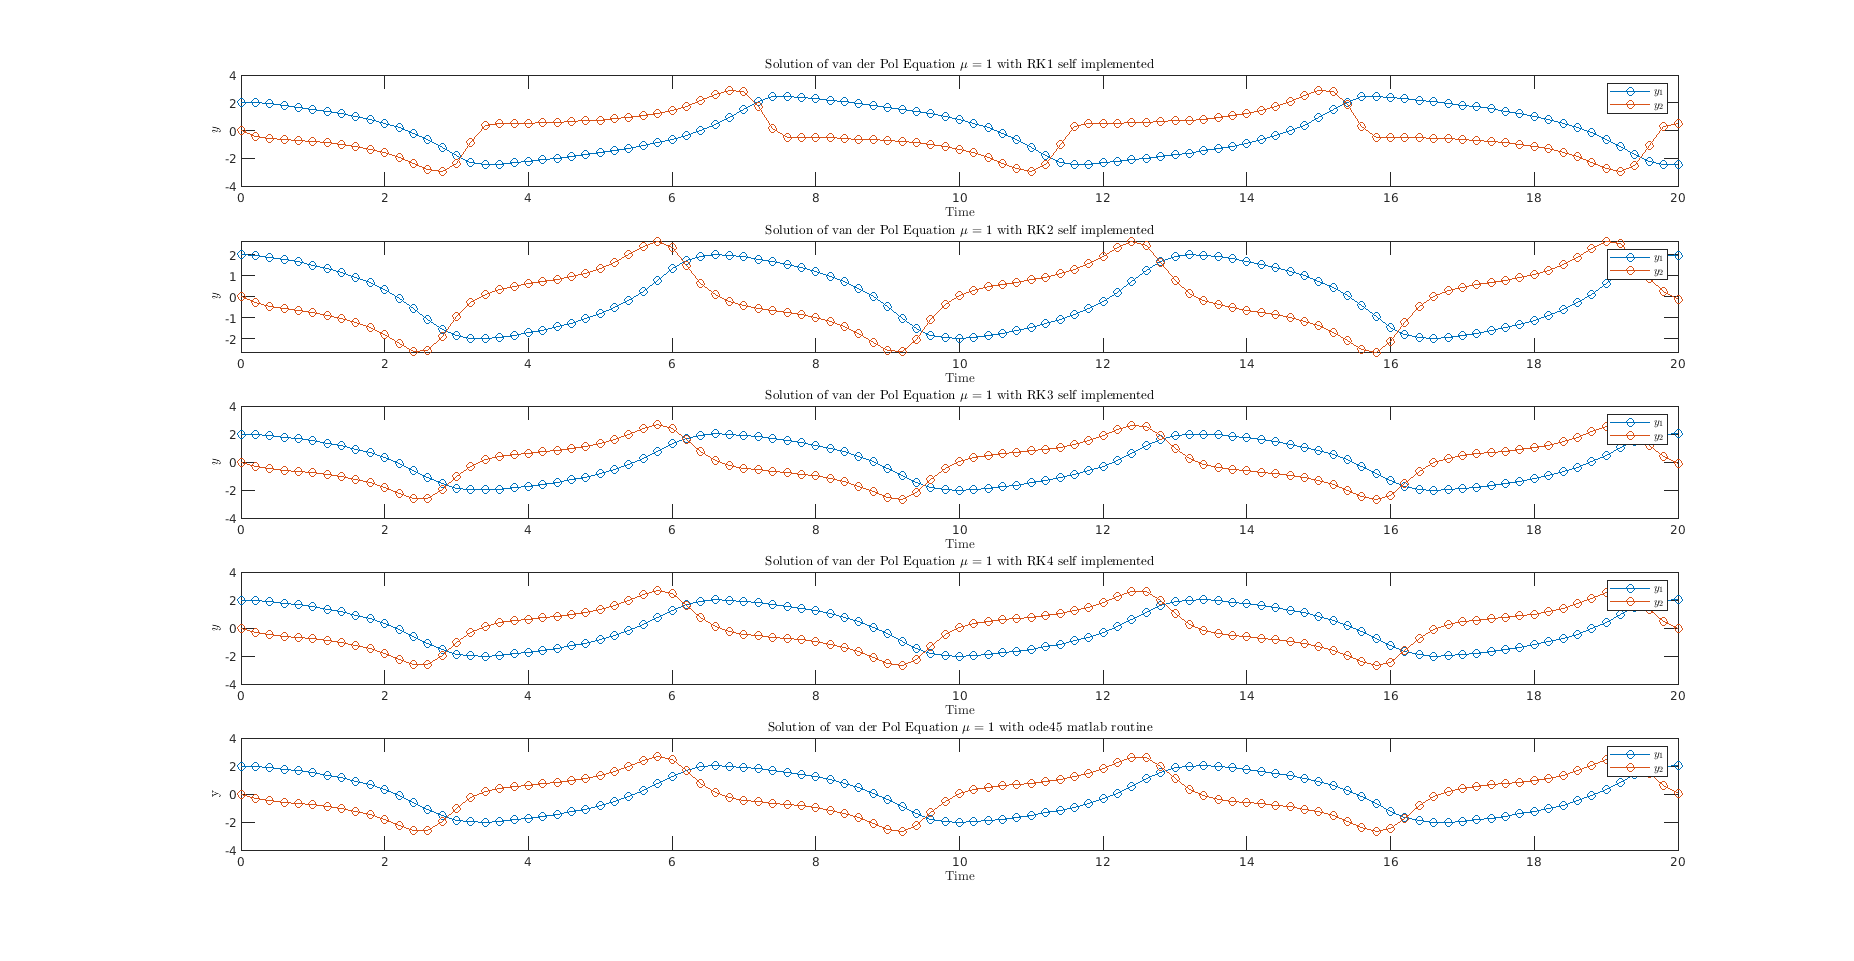
\includegraphics[width = \textwidth]{Figures/Rk.png}
    \caption{Comparison between RK1:4 and Ode45}
    \label{fig:RK1_4}
\end{figure}
The error obtained between two regimes are provided in figure \ref{fig:error}.

\begin{figure}[H]
    \centering
    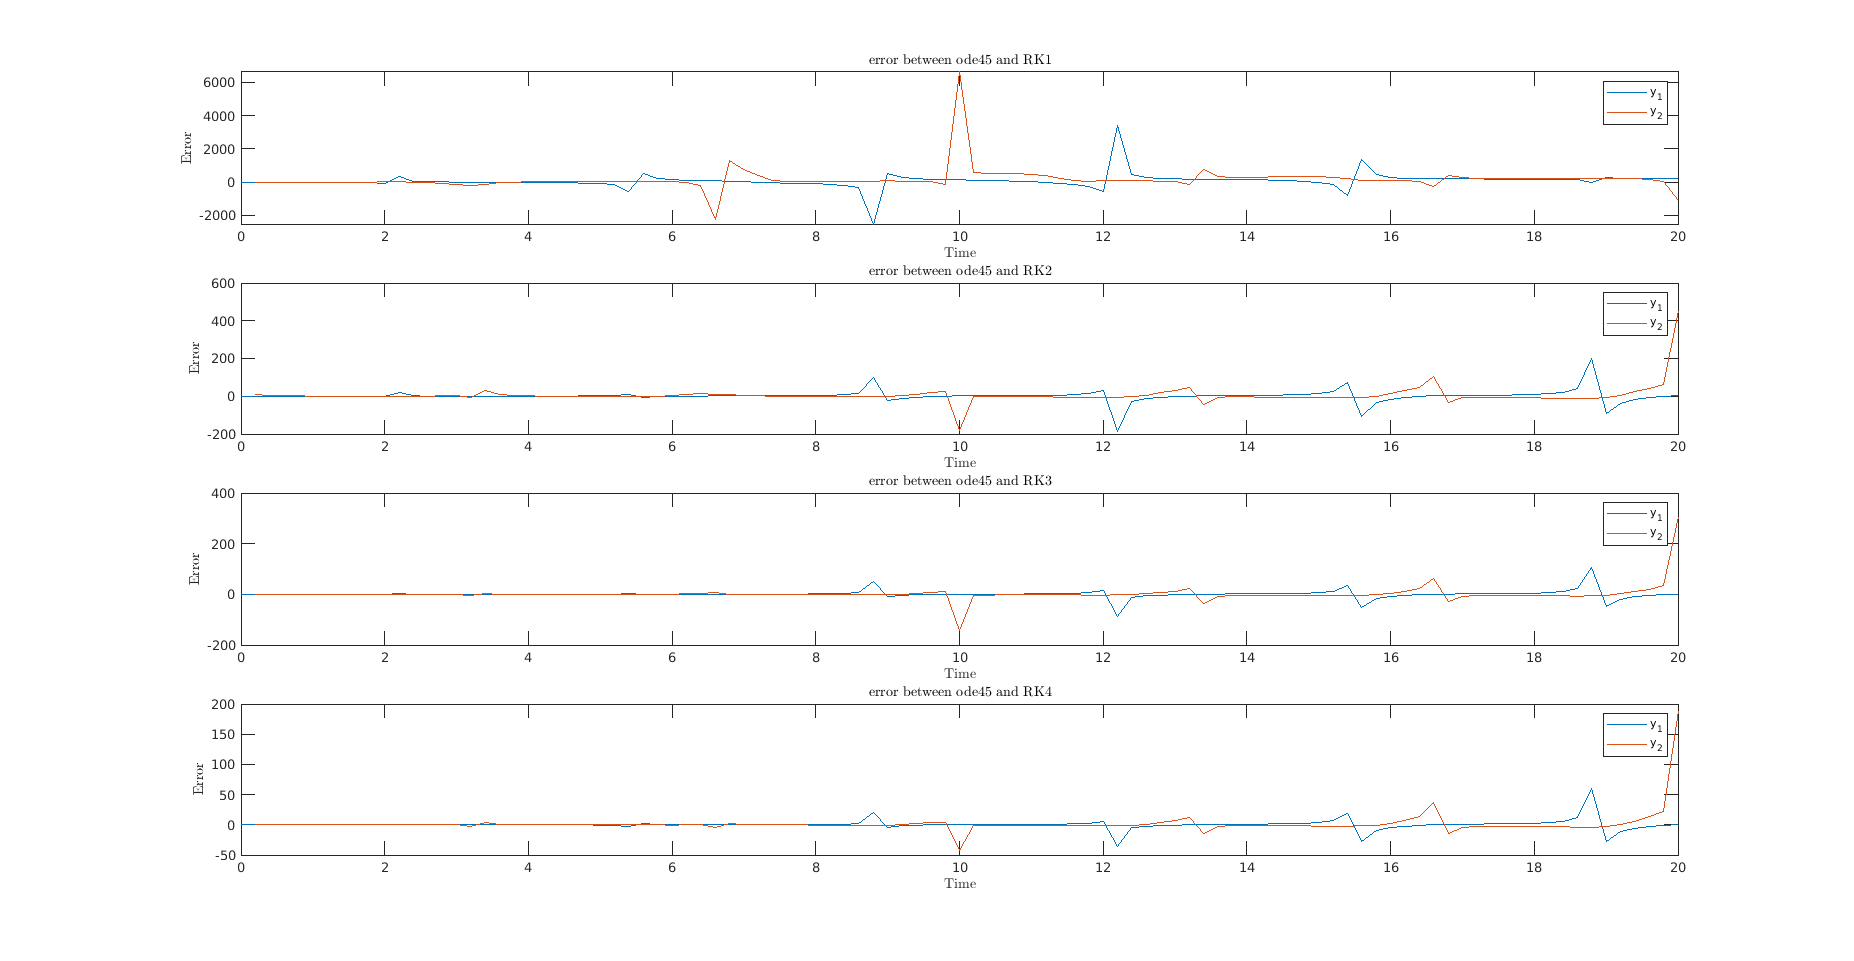
\includegraphics[width = \textwidth]{Figures/Error.png}
    \caption{Error between RK1:4 and Ode45}
    \label{fig:error}
\end{figure}
It is obvious how RK4 is the best to be used.

\subsection{General Runge-Kutta method}
More elaborated RK methods are possible. They aim at either reduce the error and/or increase stability. They take the general form
\begin{equation} \label{eqn:39}
\mathbf{x}_{n+1}=\mathbf{x}_{n}+\Delta t \sum_{i=1}^{s} b_{n} k_{n}
\end{equation}
where
\begin{equation} \label{eqn:40}
    k_{n}=f\left(t_{n}+\Delta t \cdot c_{n}, \mathbf{x}_{n}+\Delta t \sum_{j=1}^{s} a_{i j} k_{j}\right)
\end{equation}


\subsection{Adaptive Step Size Runge-Kutta Method}

There are methods for automatically adjusting the step size. They entail combining two adjacent-order RK methods into one and estimating the truncation error in the lower order solution using the difference between the higher and lower order solutions. To keep the truncation error within bounds, the step size $h$ is adjusted \cite{curtis2013orbital}. 

The integrating of RK4 into RK5 to generate the RKF4(5) method is a common example. The F is added to recognise E. Fehlberg's contribution to this RK method extension. The procedure is divided into six phases, and the Fehlberg coefficients are calculated at each stage \cite{fehlberg1969low}.


\begin{equation}
\begin{aligned}
&\mathbf{a}=\left\[\begin{bmatrix}
0 \\
1 / 4 \\
3 / 8 \\
12 / 13 \\
1 \\
1 / 2
\end{bmatrix}\right\] \quad \mathbf{b}=\left[\begin{array}{ccccc}
0 & 0 & 0 & 0 & 0 \\
1 / 4 & 0 & 0 & 0 & 0 \\
3 / 32 & 9 / 32 & 0 & 0 & 0 \\
1932 / 2197 & -7200 / 2197 & 7296 / 2197 & 0 & 0 \\
439 / 216 & -8 & 3680 / 513 & -845 / 4104 & 0 \\
-8 / 27 & 2 & -3544 / 2565 & 1859 / 4104 & -11 / 40
\end{array}\right]\\
\end{aligned}
\end{equation}
\begin{equation}
\mathbf{c}^{*}=\begin{bmatrix}
25 / 216 \\
0 \\
1408 / 2565 \\
2197 / 4104 \\
-1 / 5 \\
0
\end{bmatrix} \quad \mathbf{c}=\begin{bmatrix}{c}
16 / 135 \\
0 \\
6656 / 12825 \\
28561 / 56430 \\
-9 / 50 \\
2 / 55
\end{bmatrix}
\end{equation}

Using asterisks to indicate that RK4 is the lower order of the two

\begin{align}
&\mathbf{x}_{n+1}^{*}=\mathbf{x}_{n}+ \Delta t \left(c_{1}^{*} k_{1}+c_{2}^{*} k_{2}+c_{3}^{*} k_{3}+c_{4}^{*} k_{4}+c_{5}^{*} k_{5}+c_{6}^{*} k_{6}\right) \quad \text { Low order solution }(R K 4) \\
&\mathbf{x}_{n+1}=\mathbf{x}_{n}+\Delta t \left(c_{1} k_{1}+c_{2} k_{2}+c_{3} k_{3}+c_{4} k_{4}+c_{5} k_{5}+c_{6} k_{6}\right) \quad \text { High order solution }(R K 5)
\end{align}

Using equations \ref{eqn:39} and \ref{eqn:40}, the derivatives of the six stages are
\begin{equation}
\begin{aligned}
k_{1} &=f\left(t_{i}, \mathbf{x}_{i}\right) \\
k_{2} &=f\left(t_{i}+a_{2} \Delta t, \mathbf{x}_{i}+\Delta t b_{21} k_{1}\right) \\
k_{3} &=f\left(t_{i}+a_{3} \Delta t, \mathbf{x}_{i}+\Delta t\left[b_{31} k_{1}+b_{32} k_{2}\right]\right) \\
k_{4} &=f\left(t_{i}+a_{4} \Delta t, \mathbf{x}_{i}+\Delta t\left[b_{41} k_{1}+b_{42} k_{2}+b_{43} k_{3}\right]\right) \\
k_{5} &=f\left(t_{i}+a_{5} \Delta t, \mathbf{x}_{i}+\Delta t\left[b_{51} k_{1}+b_{52} k_{2}+b_{53} k_{3}+b_{54} k_{4}\right]\right) \\
k_{6} &=f\left(t_{i}+a_{6} \Delta t, \mathbf{x}_{i}+\Delta t\left[b_{61} k_{1}+b_{62} k_{2}+b_{63} k_{3}+b_{64} k_{4}+b_{65} k_{5}\right]\right)
\end{aligned}
\end{equation}
The truncation vector \textbf{e} is the difference between the higher order RK5 $\mathbf{x_{n+1}}$ and the lower order RK4 $\mathbf{x^{*}_{n+1}}$
\begin{equation}
\begin{aligned}
\mathbf{e} &=\mathbf{x}_{n+1}-\mathbf{x}_{n+1}^{*} \\
&=\Delta t \left[\left(c_{1}-c_{1}^{*}\right) k_{1}+\left(c_{2}-c_{2}^{*}\right) k_{2}+\left(c_{3}-c_{3}^{*}\right) k_{3}+\left(c_{4}-c_{4}^{*}\right) k_{4}+\left(c_{5}-c_{5}^{*}\right) k_{5}+\left(c_{6}-c_{6}^{*}\right) k_{6}\right]
\end{aligned}
\end{equation}
The scalar truncation error \textbf{e} is the largest value of the absolute values of the components of \textbf{e}
\begin{equation}
e=\text { maximum of the set }\left(\left|e_{1}\right|,\left|e_{2}\right|,\left|e_{3}\right|, \cdots,\left|e_{N}\right|\right)
\end{equation}
We established a tolerance \textit{tol} that the truncation error could not exceed. Rather than using the same $\Delta t$ for each step of the numerical integration process, we can vary the step size to keep the error \textbf{e} from exceeding \textit{tol}. A straightforward strategy for adaptive step size control is to update h after each time step using a formula derived in, for example, Bond and Allman in \cite{bond1996modern}.
\begin{equation}
h_{\text {new }}=h_{\mathrm{old}}\left(\frac{t o l}{e}\right)^{\frac{1}{p+1}}
\end{equation}
Where $p$ is the lower order in RKF--p(p+1). A factor $\varepsilon$ is added when $e<tol$, $\varepsilon$ may be 0.8 or 0.9. 
\begin{equation}
h_{\text {new }}=h_{\mathrm{old}}\cdot \varepsilon\left(\frac{t o l}{e}\right)^{\frac{1}{p+1}}
\end{equation}
The algorithm implemented in MATLAB can be found in Appendix \ref{app:sd}.

The output of the same equation given in \ref{eqn:van} is then compared with MATLAB ode45 routine for solving non-stiff ODE along alos with RK4 algorithm, the results obtained in figure \ref{fig:RK1_4}.

\begin{figure}[H]
    \centering
    \includegraphics[width = \textwidth]{Figures/Rk45.png}
    \caption{Comparison between RK4, RKF45 and Ode45}
    \label{fig:RK1_4}
\end{figure}
The edge of this variable step size numerical integration scheme is that it takes much less computational time compared to the regular RK family. 




\clearpage